% "{'classe':('PSI'),'chapitre':'dyn_cin','type':('td'),'titre':'Orthèse d\\'épaule', 'source':'Centrale Supélec PSI 2010','comp':('C1-05','C2-09'),'corrige':False}"
%\setchapterimage{bandeau}
\chapter*{TD \arabic{cptTD} \\ 
Orthèse d'épaule -- \ifprof Corrigé \else Sujet \fi}
\addcontentsline{toc}{section}{TD \arabic{cptTD} : Orthèse d'épaule -- \ifprof Corrigé \else Sujet \fi}

\iflivret \stepcounter{cptTD} \else
\ifprof  \stepcounter{cptTD} \else \fi
\fi

\setcounter{question}{0}
\marginnote{Centrale Supélec PSI 2010.}
\marginnote[1cm]{
\UPSTIcompetence[2]{C1-05}
\UPSTIcompetence[2]{C2-09}
}
\begin{marginfigure}[4cm]
\centering
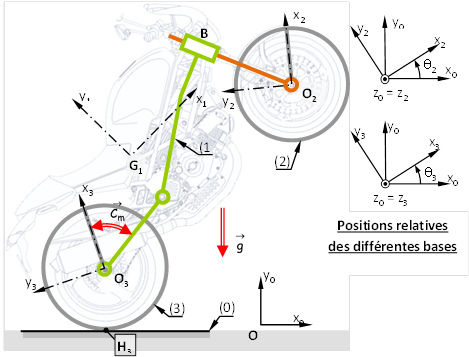
\includegraphics[width=.7\linewidth]{fig_01}
\end{marginfigure}


\subsection*{Mise en situation}

Le support de cette étude est une orthèse portable, de type exosquelette, qui contribue au développement de la tonicité musculaire de l’épaule et du bras. Installée dans le dos de l’individu
et liée à la fois au bras et à la main, elle offre une résistance aux mouvements de la main. Ainsi, le thérapeute
peut réaliser des protocoles très fins de rééducation en programmant des spectres d’efforts résistants pour chaque
mouvement du patient. Le travail du patient peut également être optimisé en le plaçant dans un environnement
de réalité virtuelle permettant de visualiser les situations de travail conçues par le thérapeute.

\begin{marginfigure}[5cm]
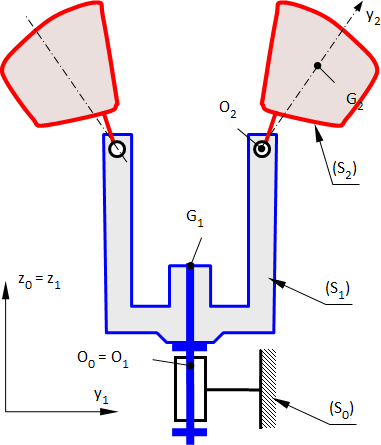
\includegraphics[width=\linewidth]{fig_02}
\end{marginfigure}
\begin{obj}
L’objectif est de mettre en place une loi de commande utilisée, par exemple, pour des
situations de travail où le patient peut déplacer le bras et doit appliquer une force prédéterminée par le
physiothérapeute, dépendante des positions des articulations. Dans le cadre de cette étude, l’effort est
élastique et caractérisé par une raideur de torsion. 
\end{obj}

La synthèse de cette loi de commande sera faite en
deux étapes : dans un premier temps, la mise en équation de l’exosquelette (limité à deux axes pour des
raisons de simplicité) sera effectuée en vue d’obtenir un modèle dynamique ; dans un deuxième temps,
la loi de commande sera déterminée en utilisant le modèle dynamique établi au préalable. Il s’agira, de
plus, de valider le dimensionnement de la chaîne de motorisation.

\footnotesize
\begin{center}
\begin{tabular}{|p{.45\linewidth}|p{.45\linewidth}|}
\hline 
Module de l'effort de manipulation maximal en régime permanent & \SI{50}{N} \\ \hline 
Compensation du couple statique (dû à la pesanteur) & Totale \\ \hline 
Raideurs $(K_1,K_2)$ de maintien (pour ce critère, seule la force $Z_F$ est
considérée). & $|\Delta Z_F/\Delta \gamma|=K_1\geq \SI{500}{N.rad^{-1}} (\pm 5\%)$ \\
& $|\Delta Z_F/\Delta \delta|=K_2\geq \SI{500}{N.rad^{-1}} (\pm 5\%)$ \\\hline 
\end{tabular}
\end{center}

\normalsize

L’actionneur ne peut fournir, en régime permanent, sur l’axe de l’articulation qu’un
couple de module inférieur à \SI{50}{Nm}. On suppose, de plus, qu’en régime transitoire le couple maximal peut
atteindre quatre fois la valeur maximale autorisée en régime permanent.
On s’intéresse ici à une situation de travail où les relations entre les variations des positions angulaires du
bras et de l’avant bras ($\gamma$ et $\delta$) et la variation de la force $Z_F$ (ces grandeurs seront définies par la suite) exercée par le patient sont équivalentes à des raideurs de torsion de valeurs $(K_1,K_2)$.

La structure de commande retenue est représentée par le schéma de la figure suivante où :
\begin{itemize}
\item $q$ et $\dot{q}$ sont respectivement les vecteurs des angles et des vitesses angulaires des articulations;
\item une boucle externe génère les trajectoires (positions, vitesses et accélérations) et éventuellement un contexte
de travail;
\item une boucle interne (de loi non linéaire) génère les couples souhaités sur chaque axe (articulation) à partir
des mesures des angles et des vitesses angulaires des articulations et éventuellement des données issues du
générateur de trajectoire ;
\item un ensemble d’actionneurs fournit les couples, sur les axes des articulations, identiques aux couples de
référence $C_a = C_{\text{ref}}$.
\end{itemize}

\begin{center}
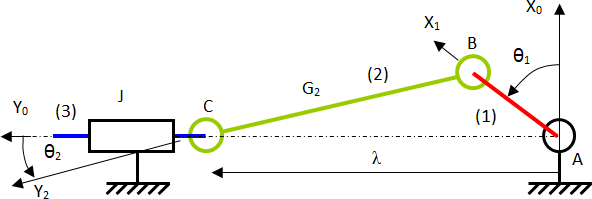
\includegraphics[width=\linewidth]{fig_03}
\end{center}


\subsection*{Modélisation dynamique «deux axes» de l’exosquelette}
\begin{obj}
Le but de cette partie est d’établir un modèle dynamique du bras et de l’avant-bras dans un plan vertical
donné. Ces deux ensembles sont soumis aux actions de la pesanteur, des couples des deux moteurs montés
dans le bras et de la force extérieure exercée sur l’extrémité de l’avant-bras. Le cadre de l’étude se limite
aux mouvements de deux axes (les deux autres axes étant supposés fixes).
\end{obj}

Le système étudié se réduit donc à l’ensemble \{Bras + Avant-bras\} relativement au reste du dispositif supposé
fixe : on suppose que les angles d’abduction/adduction et de rotation interne/rotation externe de l’épaule sont
maintenus identiquement nuls par l’action des moteurs situés dans la partie dorsale du dispositif (non étudiée
ici). Le paramétrage se réduit donc à la situation de la figure suivante qui représente l’ensemble étudié dans un plan
$\left(\vect{x};\vect{z} \right)$ donné, où l’on choisit $\vect{z}$ vertical dans le sens descendant. Le tableau précise les différents
paramètres utiles pour le calcul de dynamique envisagé.

\begin{center}
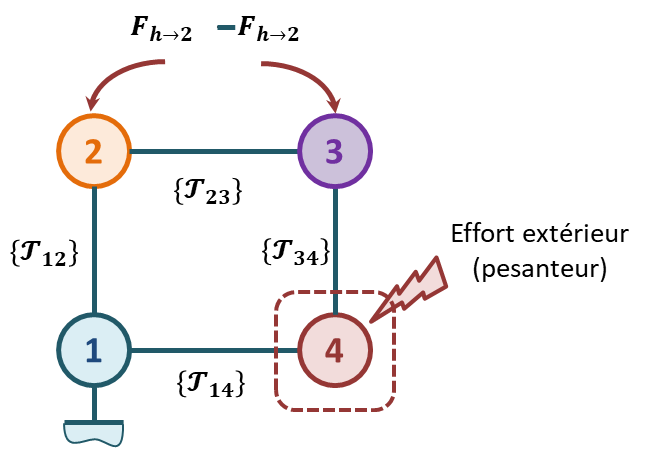
\includegraphics[width=\linewidth]{fig_04}
\end{center}


\begin{center}
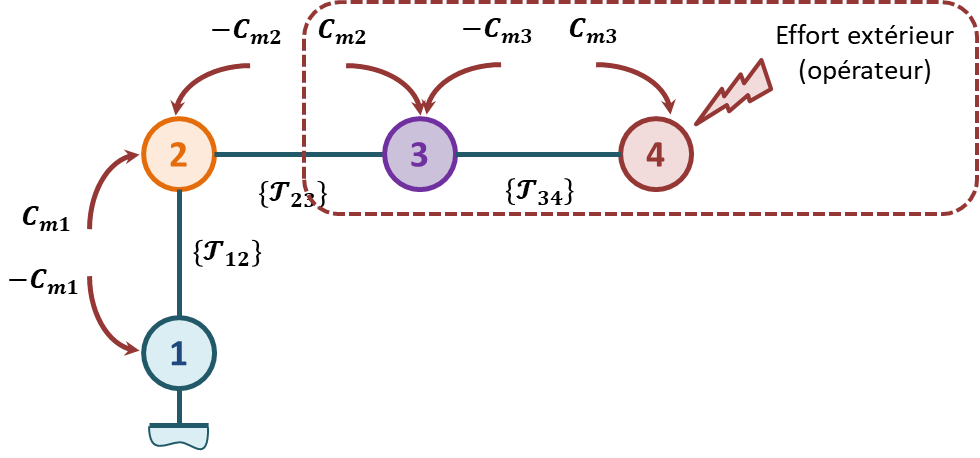
\includegraphics[width=\linewidth]{fig_05}
\end{center}


\question{Exprimer littéralement, au point $G_2$ et dans le repère $R_1$, le torseur dynamique du mouvement du solide
\{Avant-bras\} par rapport au référentiel fixe $R_0$ supposé galiléen : $\torseurdyn{\text{Avant-bras}}{R_0}_{G2,\base{x_1}{y_1}{z_1}}$.}

Les différentes actions mécaniques agissant sur le dispositif sont les suivantes :
\begin{itemize}
\item l’action de la pesanteur sur les solides \{Bras\} et \{Avant-bras\} ;
\item l’action du bâti sur le solide \{Bras\} au travers de la liaison pivot d’axe $\axe{O}{y}$ et de torseur d’action mécanique écrit sous la forme générique suivante : 
$\torseurstat{T}{\text{Bâti}}{\text{Bras}}=\torseurl{X_1\vect{x_1}+Y_1\vect{y_1}+Z_1\vect{z_1}}{L_1\vect{x_1}+M_1\vect{y_1}+N_1\vect{z_1}}{O}$ où les paramètres $\left(X_1, Y_1, Z_1, L_1, M_1, N_1\right)$ sont inconnus;
\item l’action du premier actionneur sur le solide \{Bras\} :
$\torseurstat{T}{\text{Actionneur 1}}{\text{Bras}}=\torseurl{\vect{0}}{C_1(t) \vect{y}}{O}$ où le couple $C_1(t)$ exercé est connu au cours du temps;
\item  l’action du solide \{Bras\} sur le solide \{Avant-bras\} au travers de la liaison pivot d’axe $\axe{A}{y}$ et de torseur d’action mécanique écrit sous la forme générique suivante : 
$\torseurstat{T}{\text{Bras}}{\text{Avant-bras}}=\torseurl{X_2\vect{x_1}+Y_2\vect{y}+Z_2\vect{z_1}}{L_2\vect{x_1}+M_2\vect{y}+N_2\vect{z_1}}{A}$ où les paramètres $\left(X_2, Y_2, Z_2, L_2, M_2, N_2\right)$ sont inconnus;
\item les actions du second actionneur sur le solide \{Bras\} et le solide \{Avant-bras\}, respectivement notées :
$\torseurstat{T}{\text{Actionneur 2}}{\text{Bras}}=\torseurl{\vect{0}}{-C_2(t) \vect{y}}{A}$ et 
$\torseurstat{T}{\text{Actionneur 2}}{\text{Avant-bras}}=\torseurl{\vect{0}}{C_2(t) \vect{y}}{A}$ où le couple $C_2(t)$ exercé est connu au cours du temps;
\item l’action du patient sur l’avant-bras, modélisée par une force appliquée à l’extrémité $B$ de l’avant-bras et
définie par : 
$\torseurstat{T}{\text{Force}}{\text{Avant-bras}}=\torseurl{X_F\vect{x}+Z_F\vect{z}}{\vect{0}}{B}$. 
\end{itemize}

On veut déterminer les deux équations permettant de décrire le mouvement des deux axes de l’orthèse. On
suppose pour cela que les deux liaisons pivots sont parfaites.

Le PFD permet d'obtenir la relation suivante : 
$$
\begin{array}{ll}
C_1(t)=&
\left(B_1+B_2 +m_1 \lambda_1^2 + m_2 l_1^2 + m_2 \lambda_2^2 \right)\ddot{\gamma} +\left( B_2 + m_2\lambda_2^2\right) \ddot{\delta}\\
& +m_2 l_1 \left( \lambda_2 \left(2\ddot{\gamma}+\ddot{\delta} \right)\cos \delta + \lambda_2 \left( \dot{\gamma}^2-\left( \dot{\gamma} + \dot{\delta}\right)^2\right) \sin\delta\right) \\
& + m_1g\lambda_1\sin\gamma + m_2 g \left(l_1 \sin \gamma+\lambda_2 \sin \left(\gamma+ \delta\right) \right)\\
& -X_F \left( l_1 \cos \gamma +l_2 \cos \left( \gamma+\delta\right) \right) + Z_F \left( l_1 \sin \gamma + l_2 \left( \gamma + \delta \right)\right)
\end{array}
$$

\question{Détailler la démarche qui a permis d’obtenir cette équation, on précisera en particulier l’isolement,
le bilan des Actions Mécaniques Extérieures et le choix des équations utilisées.}
\ifprof
\begin{corrige}
\end{corrige}
\else
\fi

\question{Appliquer la démarche pour retrouver l'équation donnée.}
\ifprof
\begin{corrige}
\end{corrige}
\else
\fi

\question{Écrire une deuxième relation issue du Principe Fondamental de la Dynamique, indépendante de la
précédente, faisant intervenir le couple $C_2(t)$, et qui permette de ne pas faire apparaître les composantes $L_1$, $M_1$, $N_1$, $L_2$, $M_2$, $N_2$ des torseurs des actions de liaison. On détaillera la démarche de la même façon que lors de la première question.}

\ifprof
\begin{corrige}
\end{corrige}
\else
\fi

\question{En déduire que les deux équations précédentes peuvent s'écrire sous la forme matricielle suivante : 
$\begin{pmatrix}
C_1 \\ C_2
\end{pmatrix}
=
A
\begin{pmatrix}
\ddot{\gamma} \\ \ddot{\delta}
\end{pmatrix}
+
B
\begin{pmatrix}
\dot{\gamma} \\ \dot{\delta}
\end{pmatrix}
+
C
+
Q
\begin{pmatrix}
X_F \\ Y_F
\end{pmatrix}$ où $C$ est un vecteur et $A$, $B$ et $Q$ sont des matrices $2\times 2$ que l'on précisera en fonction des paramètres du mouvement $\left(\gamma,\delta\right)$ et de leurs dérivées premières $\left(\dot{\gamma},\dot{\delta}\right)$.
}

\ifprof
\begin{corrige}
\end{corrige}
\else
\fi


\question{Calculer les couples $(C_1,C_2)$ exercés par les actionneurs sur les axes des articulations dans le cas où
l’on n’exerce pas de force à l’extrémité du solide \{Avant-bras\} ($X_F = 0$, $Z_F = 0$) et dans une position statique. Discuter de la configuration angulaire la plus défavorable vis-à-vis du cahier des charges.}
\ifprof
\begin{corrige}
\end{corrige}
\else
\fi


\question{Compte-tenu du cahier des charges, quelle charge statique maximale peut-on exercer sur l’extrémité du solide \{Avant-bras\} ?}
\ifprof
\begin{corrige}
\end{corrige}
\else
\fi
%
%\subsection*{Synthèse d'une loi de commande << deux axes >>}
%\begin{obj}
%L’objectif de cette partie est de déterminer une loi de commande afin que la relation entre les variations
%des positions $t\left(\gamma, \delta\right)^t$ du bras et de l’avant-bras et la variation de la force $Z_F$ exercée par le patient soit
%celle d’une raideur en torsion de valeurs $(K_1;K_2)$ données dans le cahier des charges. La
%raideur comparativement à la force $X_F$ ne sera pas à vérifier dans ce cas d’étude.
%\end{obj}
%
%L’équation dynamique décrivant le comportement de l’exosquelette est de la forme
%$
%A\left(q,\dot{q}\right)\ddot{q}+
%B\left(q,\dot{q}\right)\dot{q}+
%C\left(q,\dot{q}\right)+
%Q\left(q,\dot{q}\right)\cdot F = C_a$
%où $C_a=\left( C_1 \; C_2\right)^t$, $q=\left( \gamma \; \delta\right)^t$ et 
%$F=\left( X_F \;  Z_F\right)^t$. On note sous forme vectorielle $q_{\text{ref}}= \left( \gamma_{\text{ref}}\; \delta_{\text{ref}}\right)^t$ les consignes
%de positions angulaires. La loi de commande adoptée est organisée selon deux boucles :
%\begin{itemize}
%\item une boucle externe linéaire ;
%\item une boucle interne non linéaire qui détermine le couple $C_a$ par la relation
%$ C_a =
%A\left(q,\dot{q}\right)U+
%B\left(q,\dot{q}\right)\dot{q}+
%C\left(q,\dot{q}\right)+
%$
%où $U = (U_1 \; U_2)^t$ sont les deux nouvelles commandes issues du correcteur linéaire de la boucle externe. 
%\end{itemize}
%Le principe de cette loi de commande est donné par la structure représentée par le schéma de la figure suivante.
%
%
%\begin{center}
%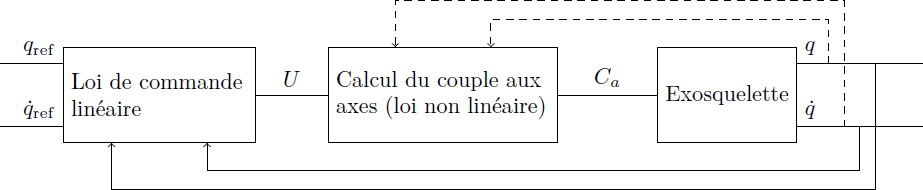
\includegraphics[width=\linewidth]{fig_06}
%\end{center}
%
%%
%%\question{}
%%\textit{Donner au moins un argument, en particulier vis-à-vis du cahier des charges souhaité, de l’intérêt de la boucle interne correspondant à la loi non linéaire donnée précédemment.}
%%\ifprof
%%\begin{corrige}
%%\end{corrige}
%%\else
%%\fi
%
%
%Pour la synthèse de la loi de commande, il est nécessaire de linéariser le modèle dynamique autour d’un point
%de fonctionnement défini par les positions articulaires $(\gamma_0 \; \delta_0)^t$  et les forces $\left(X_{F0} \; Z_{F0}\right)^t$ . On note autour de ce
%point de fonctionnement :
%\begin{itemize}
%\item $u = \left(u_1 \; u_2\right)^t$ les variations des grandeurs de commande autour de $U_0 = \left(U_{10} \; U_{20}\right)^t$  ;
%\item $q_1 = \left(\gamma_1 \; \delta_1\right)^t$ les variations des positions angulaires des deux articulations autour de $q_0 = \left(\gamma_0\; \delta_0\right)$ ;
%\item $f = \left(x_F \; z_F \right)$ les variations des efforts exercés par le patient autour de $F_0=\left(X_{F0} \; Z_{F0}\right)^t$.
%\end{itemize}
%En utilisant la loi correspondant à la boucle interne, le modèle dynamique peut être réécrit selon la forme 
%$\ddot{q}=I+N\left(q,\dot{q},F \right)$ où $N\left(q,\dot{q},F \right)=\text{M}\left(q,\dot{q}\right)\cdot F$.
%
%\question{}
%\textit{Préciser l’expression de la matrice M en fonction de A et de Q.}
%\ifprof
%\begin{corrige}
%\end{corrige}
%\else
%\fi
%
%\question{}
%\textit{Donner, par exemple sous forme algorithmique, une démarche permettant de linéariser le modèle dynamique
%selon la forme 
%$\ddot{q}_1=\tilde{\text{A}}q_1 + \tilde{\text{B}}\dot{q}_1 + \tilde{\text{G}}u + \tilde{\text{H}}f$ où $\tilde{\text{A}}$, $\tilde{\text{B}}$, $\tilde{\text{G}}$ et $\tilde{\text{H}}$ sont des matrices constantes, éventuellement dépendantes du point de fonctionnement.}
%
%La démarche de linéarisation fait intervenir $\dfrac{\partial N}{\partial q}$, $\dfrac{\partial N}{\partial \dot{q}}$ et $\dfrac{\partial N}{\partial F}$. L'expression explicite du modèle linéarisé en fonction de $M$ n'est pas demandée.
%\ifprof
%\begin{corrige}
%\end{corrige}
%\else
%\fi
%

%\question{}
%\textit{}
%\ifprof
%\begin{corrige}
%\end{corrige}
%\else
%\fi




\ifprof
\else
\begin{marginfigure}
\centering

\includegraphics[width=3cm]{Cy_04_02_TD_01_Orthese_PFD_qr}
\end{marginfigure}
\fi

\ifprof

\question{}
\begin{center}
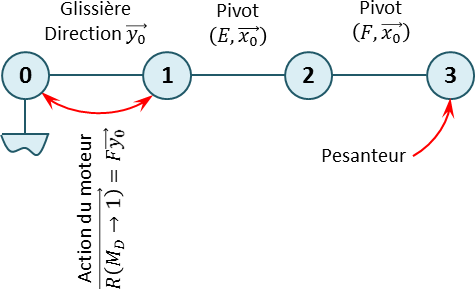
\includegraphics[width=\linewidth]{cor_01}
\end{center}

\question{}
\begin{center}
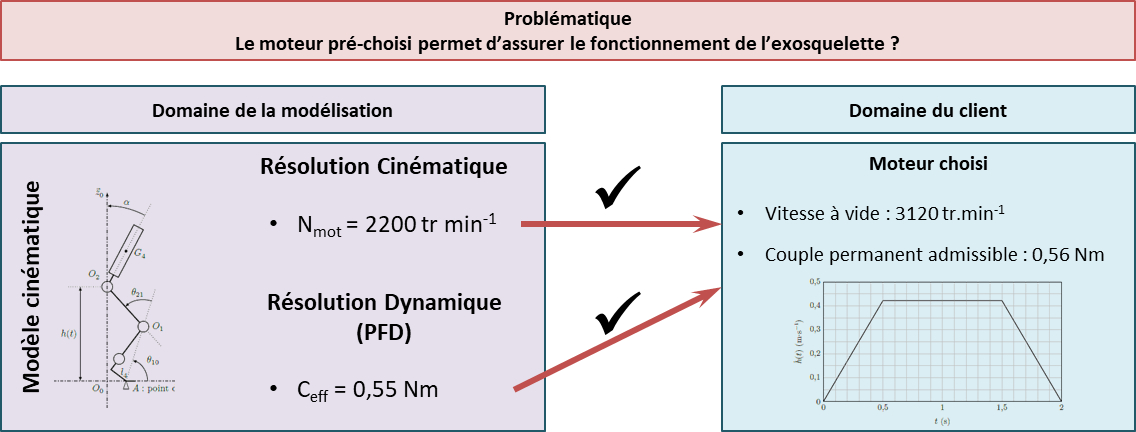
\includegraphics[width=\linewidth]{cor_02}
\end{center}

\question{}
\begin{center}
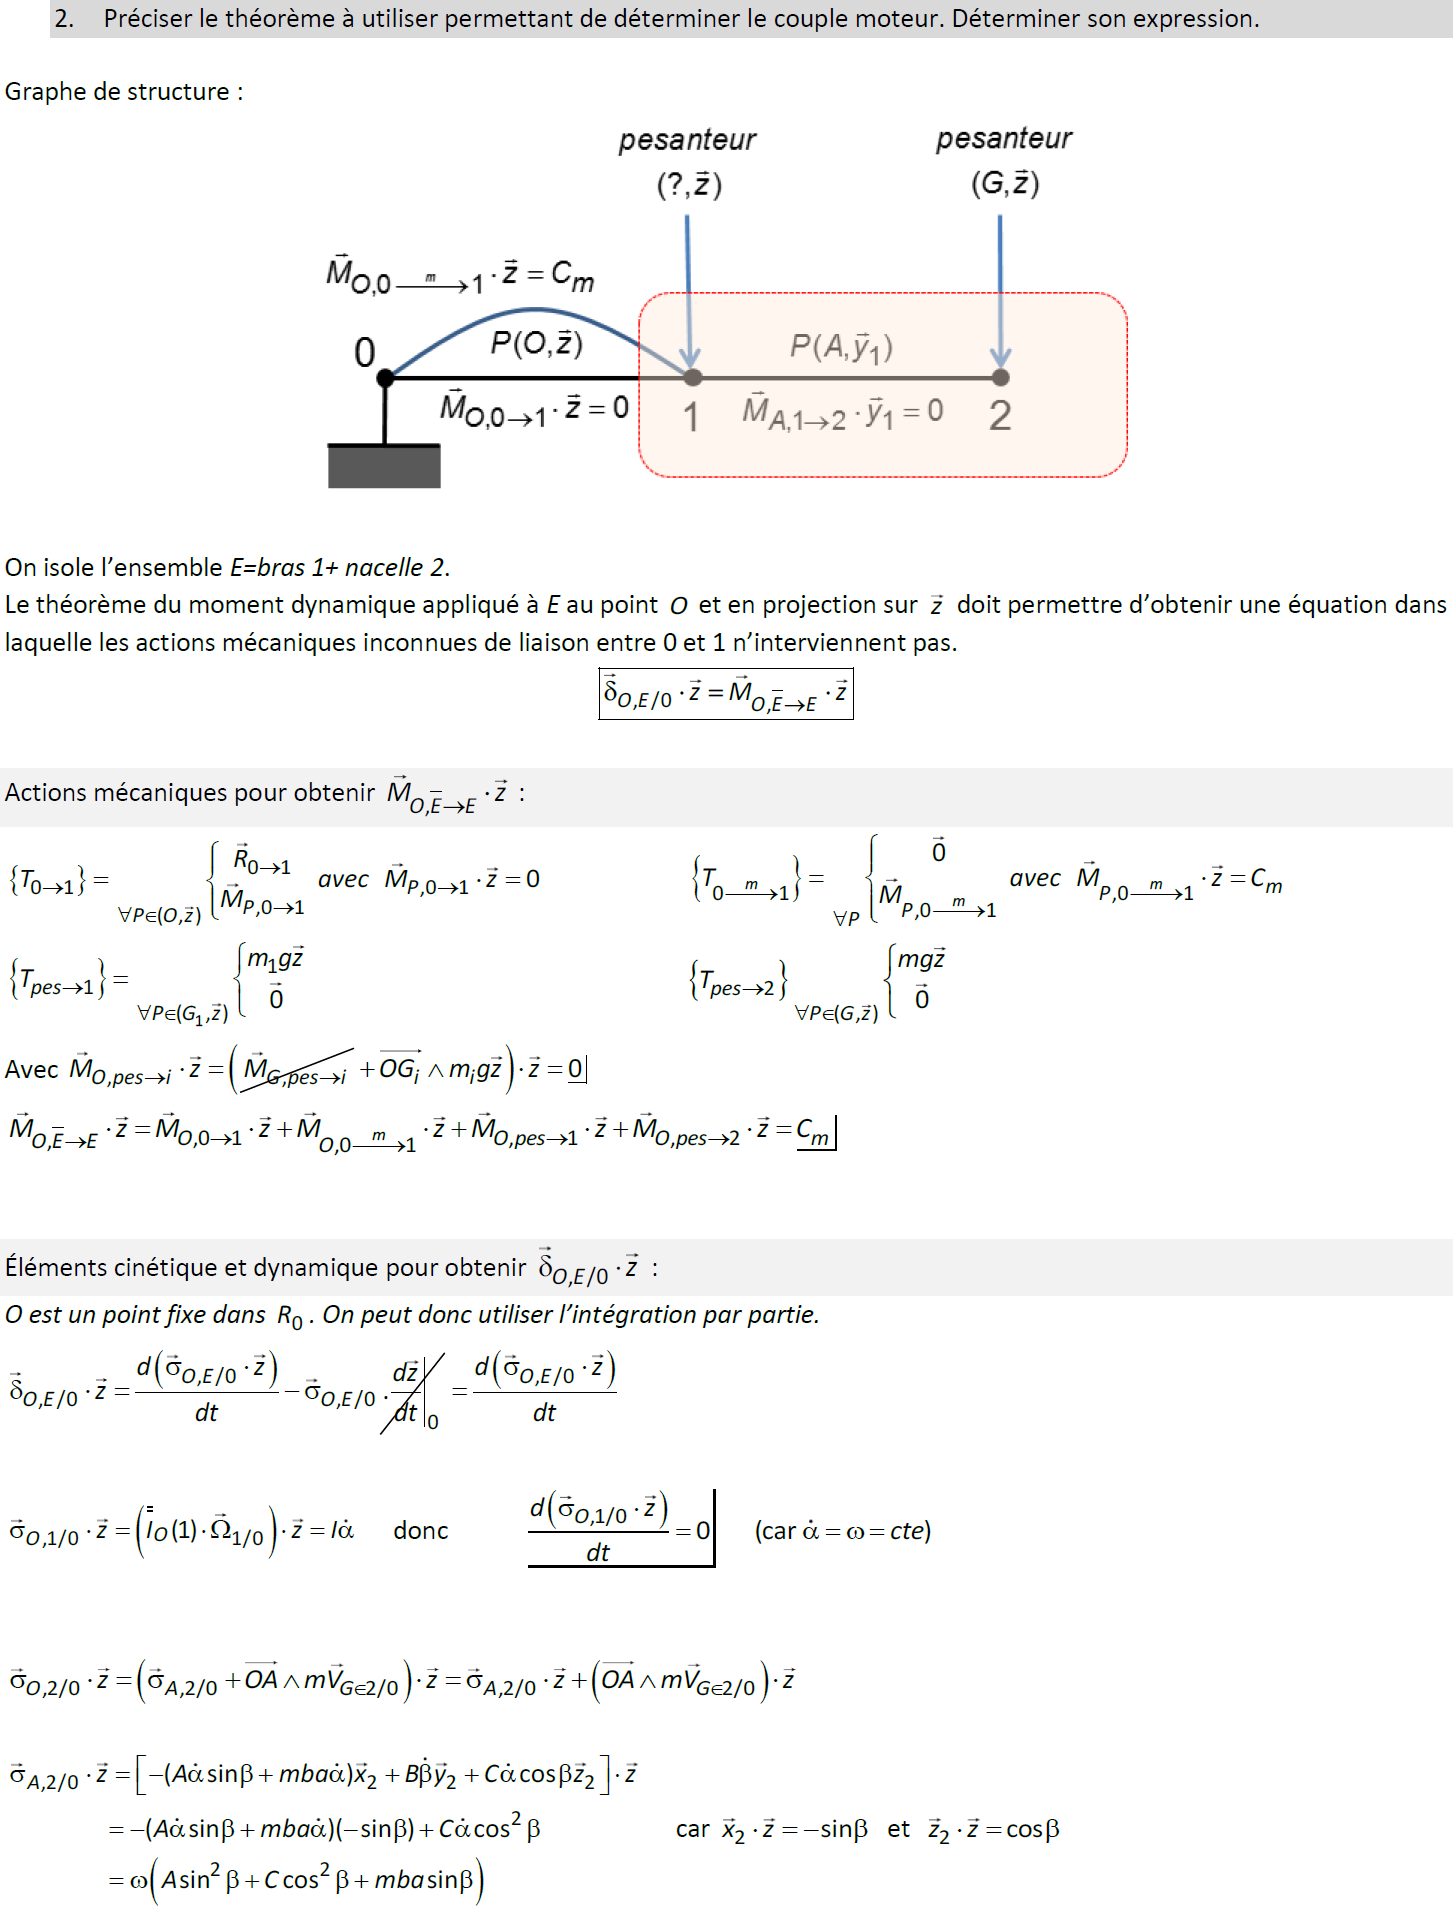
\includegraphics[width=\linewidth]{cor_03}
\end{center}

\question{}
\begin{center}
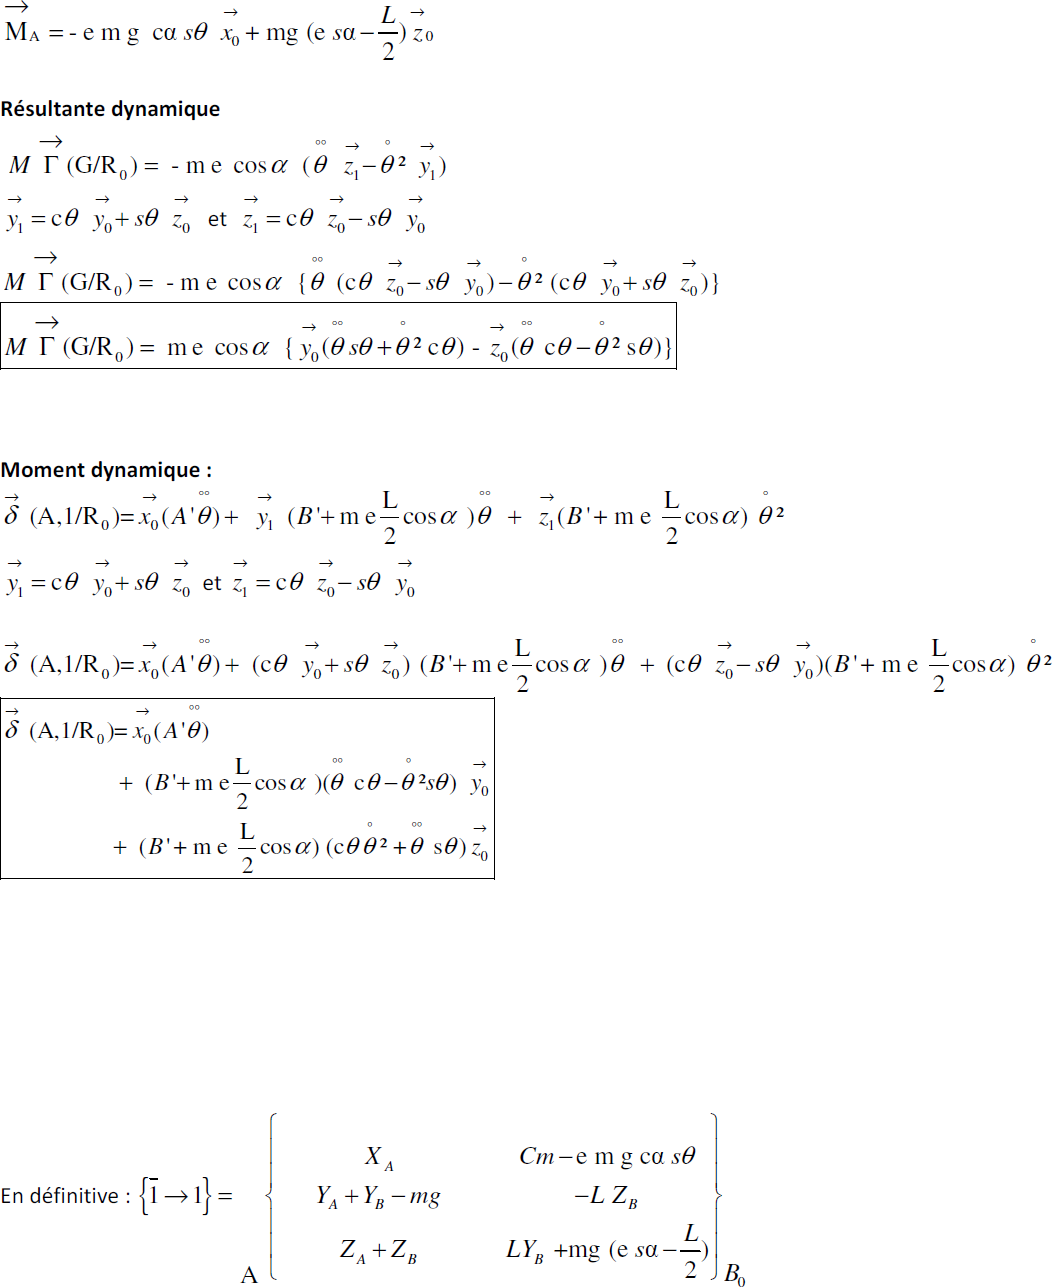
\includegraphics[width=\linewidth]{cor_04}

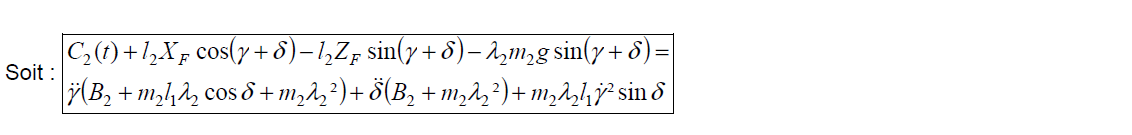
\includegraphics[width=\linewidth]{cor_04_bis}
\end{center}

\question{}
\begin{center}
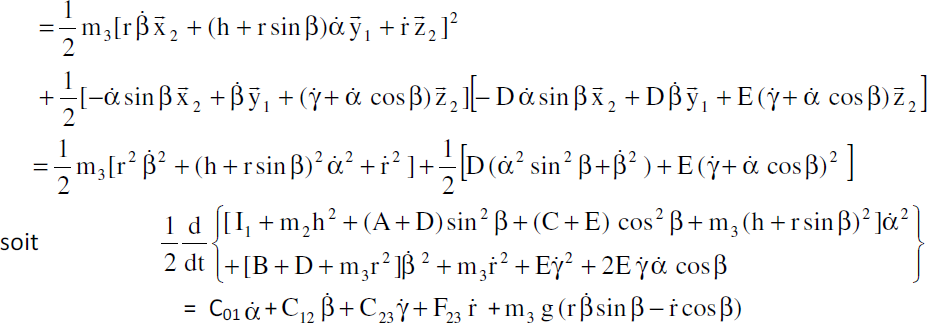
\includegraphics[width=\linewidth]{cor_05}
\end{center}

\question{}
\begin{center}
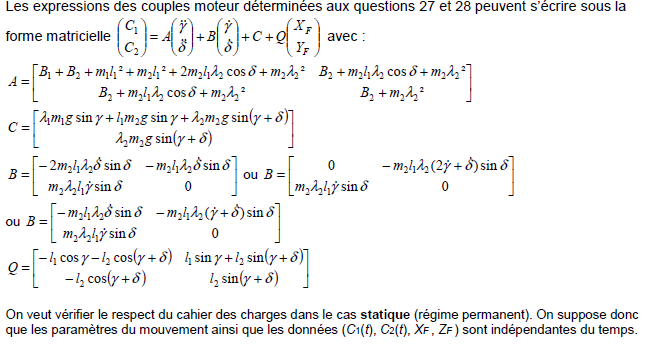
\includegraphics[width=\linewidth]{cor_06}
\end{center}

\question{}
\begin{center}
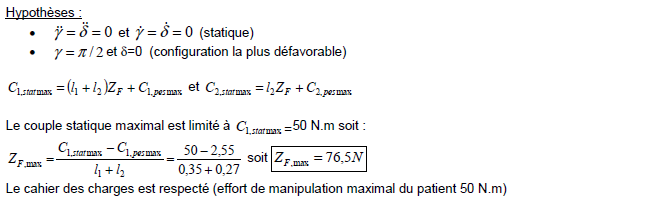
\includegraphics[width=\linewidth]{cor_07}
\end{center}
%
%\question{}
%\begin{center}
%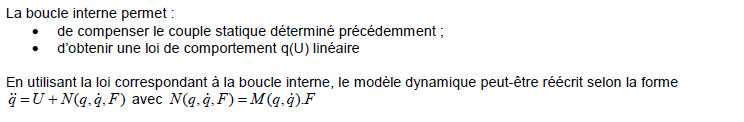
\includegraphics[width=\linewidth]{cor_08}
%\end{center}
%
%\question{}
%\begin{center}
%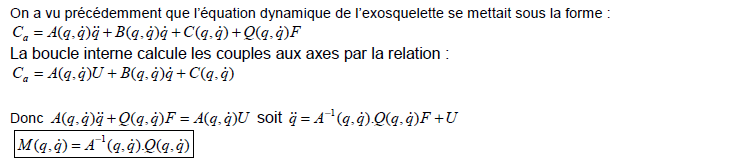
\includegraphics[width=\linewidth]{cor_09}
%\end{center}
%
%\question{}
%\begin{center}
%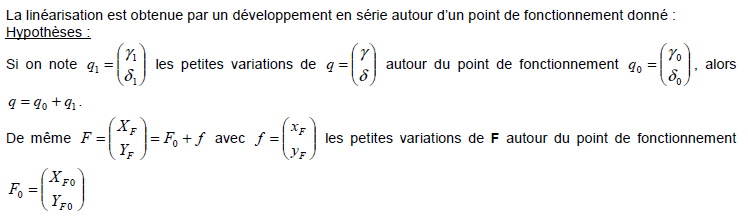
\includegraphics[width=\linewidth]{cor_10_1}
%
%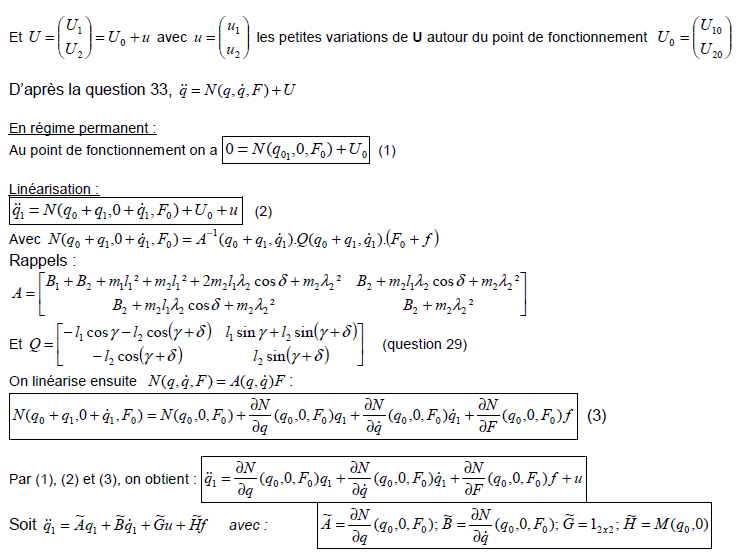
\includegraphics[width=\linewidth]{cor_10_2}
%\end{center}

\else
\fi
